\chapter{TINJAUAN PUSTAKA}

\section{Light Scattering}
Cahaya merupakan gelombang elektromagnetik yang memiliki sifat layaknya partikel. Dengan adanya
dualisme gelombang dan partikel tersebut membuat nanopartikel dapat membelokan arah gerak dari
cahaya tersebut. Apabila cahaya dihamburkan oleh partikel dapat menyebabkan fenomena yang disebut
dengan pemantulan, pembiasan atau difraksi. Pada saat berkas cahaya terhamburkan oleh partikel,
intensitas dari cahaya yang diteruskan akan berkurang. Peristiwa ini merupakan peristiwa penghamburan
cahaya atau \textit{light scattering}\cite{Black1996}.

Pada \textit{Static Light Scattering} intensitas dari cahaya yang terhamburkan  akan dianalisa dalam
bentuk intensitas terhadap waktu yang dimana informasi ini dapat dimanfaatkan untuk pengukuran berat
molekular, komposisi oligomeric, dan jari-jari dari makromolekul tersebut. Selain itu, dari data
tersebut dapat digunakan sebagai acuan untun mengukur konformasi kasar dari sebuah protein. Oleh
karena itu metode \textit{Light Scattering} ini dapat juga digunakan untuk menganalisa struktur dari
sebuah virus\cite{Stetefeld2016}

Sistem dari penghamburan cahaya tidak selalu berbasis molekul. Pada dasarnya sendiri pada saat
sebuah objek terkena cahaya, objek tersebut dapat memantulkan atau membelokan arah cahaya tersebut.
Oleh karena itu dalam \textit{Light Scattering}, cahaya dari laser tidak akan terlihat oleh mata
apabila tidak terpantulkan oleh sebuah partikel lainnya. Hal tersebutlah yang menyebabkan mengapa
langit berwarna biru. Cahaya laser yang terlihat oleh mata kita merupakan hasil dari hamburan
partikel di sekitar arah gerak cahaya tersebut.



\section{Dynamic Light Scattering}
Partikel tidak sepenuhnya dalam kondisi diam. Terutama partikel yang tersuspensi dimana terdapat
medium lainnya yang membuat partikel tersebut berfluktuasi dari waktu ke waktu. Dari fluktuasi
intensitas terhadap waktu didapatkan informasi berupa solusi persamaan dinamika. Analisa terhadap
rata rata intensitas yang didapatkan disebut dengan \textit{Static Light Scattering} (SLS) sedangkan
kumpulan data hasil dari fluktuasi partikel tersebut disebut dengan \textit{Dynamic Light Scattering}
(DLS).

Metode DLS memanfaatkan hamburan elektromagnetik dari partikel yang terdispersi. Medan elektrik
dari komponen pada gelombang cahaya laser berinteraksi dengan molekul sampel dengan adanya osilasi
dipol elektrik terhadap molekul sampel pada frekuensi yang sama yang menghasilkan emisi cahaya.
Cahaya akan terhamburkan ke berbagai arah sembari mempertahankan energi konstan dari foton. 

Sebagai contoh, pada sampel yang seringkali digunakan pada biokimia untuk mengidentifikasi sebuah
protein yang dimana lebih kecil dibandingkan dengan panjang gelombang dari laser pada DLS itu
sendiri ( $<0.1\lambda$ ) sehingga cahaya dapat tembus dan terjadi hamburan isotropic seperti yang
dijelaskan pada hukum \textit{Rayleigh Scattering}, yaitu merupakan penyebaran radiasi
elektromagnetik dari keadaan elektron yang terikat setelah foton tereksitasi ke keadaan yang jauh
dari resonansi\cite{Piazza2005}.

Partikel terdispersi dalam suatu medium akan mengikuti sebuah pola pergerakan acak yang disebut
dengan gerak Brown. Pada gerak brown, digunakan persamaan \textit{Stokes-Einstein} untuk
menghubungkan gerak Brownian dengan ukuran dari partikel\cite{Anindya2018}. Persamaan dari
\textit{Stokes-Einstein} dapat dituliskan sebagai berikut.
\begin{equation}
    D = \frac{k_b T}{6 \pi \eta R}
\end{equation}

Dalam hamburan cahaya, ketika laser mengenai molekul, cahaya yang terhamburkan akan menyebar ke
segala arah dan intensitas dari hamburan tersebut akan terdeteksi oleh detector. Cahaya monokromatik
yang terdeteksi akan mengalami pelebaran Doppler karena pergerakan fluktuatif dari molekul tersebut.
Cahaya yang tersebar akan menghasilkan fase yang saling meniadakan atau membangun sinyal yang dapat
dideteksi. Akibat adanya fluktuasi tersebut, nilai yang didapatkan dari detektor akan berubah-ubah
seiring waktu. Oleh karena itu pada DLS pengukuran berdasarkan dari nilai distribusi dari gerak
Brownian\cite{Falke2019,Pavan2022}. 




\section{Fotodioda}
Pada umumnya, sensor merupakan perangkat yang merubah stimulus yang masuk ke dalam sensor menjadi
suatu sinyal dalam bentuk arus. Sensor cahaya berdasarkan perubahan elektrik yang dihasilkan dibagi
menjadi dua jenis, yaitu fotovoltaik dan fotokonduktif. Salah satu sensor cahaya jenis fotokonduktif
adalah sensor fotodioda. Sensor fotodioda dapat merespon stimulus berupa cahaya tampak maupun tidak
tampak dan mengkonversi intensitas cahaya yang terdeteksi menjadi arus\cite{Setyaningsih2017}.

\begin{figure}[H]
    \centering
    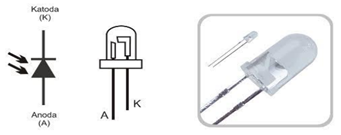
\includegraphics{Images/Fotodioda.png}
    \caption{Lambang dan Gambar Fotodioda LED Inframerah}
    \label{fig:led photodiode}
\end{figure}

Fotodioda adalah suatu jenis dioda yang resistansinya akan berubah-ubah apabila terkena sinar
cahaya. Resistansi dari fotodioda dipengaruhi oleh intensitas cahaya yang diterimanya, semakin
banyak cahaya yang diterima maka semakin kecil resistansi dari fotodioda dan begitupula sebaliknya
jika semakin sedikit intensitas cahaya yang diterima oleh sensor fotodioda maka semakin besar nilai
resistansinya\cite{Setyaningsih2017,Arta2020}.

Pada fotodioda, terdapat bahan semikonduktor seperti \textit{silicon} (Si) atau \textit{gallium
arsenide} (GaAs) dan lain lain seperti \textit{indium antimonide} (InSb), \textit{lead selenide}
(PbSe) dan \textit{timah sulfida} (PbS). Fotodioda memiliki lapisan substrat dengan area depletion
sebagai tempat masuknya foton. Pada saat foton masuk ke area depletion, elektron pada N-substrat
akan bergerak membuat pasangan lubang-elektron pada katoda sehingga terjadi arus listrik pada
rangkaian fotodioda\cite{Vlasov2023}.

\begin{figure}[H]
    \centering
    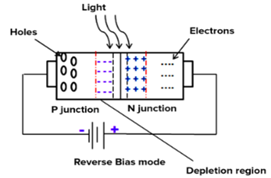
\includegraphics{Images/Bias Fotodioda.png}
    \caption{P-N Fotodioda}
    \label{fig:p-n photodiode}
\end{figure}

Pada prinsipnya fotodioda menghasilkan arus proporsional dari cahaya yang mengenai area aktif dari
fotodioda. Kebanyakan aplikasi dari pengukuran sensor ini menggunakan transimpedance amplifier
untuk mengkonversi nilai arus menjadi keluaran voltase. Adanya amplifier tersebut dapat
mengoperasikan fotodioda dalam mode \textit{photovoltaic} dimana op amp akan membuat voltase di
sekitar fotodioda pada 0V. Sebagai contoh terdapat pada OPT101 yang digunakan pada percobaan kali
ini.

\begin{figure}[H]
    \centering
    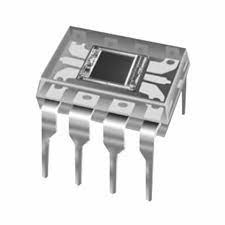
\includegraphics[width=5cm]{Images/OPT101.jpg}
    \caption{Fotodioda dengan \textit{Transimpedance Amplifier} OPT101}
    \label{fig:opt101}
\end{figure}



\section{Mikrokontroler}
Mikrokontroler merupakan perangkat yang memiliki mikro prosesor dengan memori program dan memori
serbaguna, lalu didukung oleh fasilitas pendukung lainnya seperti output berupa data ke display
layaknya komputer dalam sebuah satu chip komputer sehingga mikrokontroler biasa disebut dengan
\textit{single chip computer}. Mikrokontroler ini dapat mengkontrol atau mengendalikan sebuah sistem
yang telah diprogram dalam chip tersebut. Berbeda dengan mikroprosesor dimana dalam mikrokontroler
ini terdapat komponen mikroprosesor yang didukung ADC, PPL, dan EEPROM dalam satu kemasan
\cite{Sokop2016}.

Dalam penelitian ini mikrokontroler yang digunakan merupakan mikrokontroler Arduino yang merupakan
platform komputasi fisik berbasiskan open source yang memiliki rangkaian input/output sederhana
dalam mengimplementasikan bahasa processing. Rangkaian ini memiliki IDE (\textit{Integrated 
Development Environment}) yang bersifat open source sehingga komponen dapat terhubung dengan
komponen lainnya tanpa bantuan alat lainnya. Pada perancangannya digunakan papan Arduino Uno R3
yang merupakan board mikrokontroler yang didasasrkan pada ATmega328\cite{Sokop2016}. Spesifikasi
dari Arduino Uno R3 sendiri yaitu:
\begin{longtable}{p{6cm}p{3pt}p{6cm}}
    \hspace{20pt} Mikrokontroller &:& ATmega328\\
    \hspace{20pt} Tegangan Pengoperasian &:&5 V\\
    \hspace{20pt} Tegangan Input Rekomendasi &:& 7-12V\\
    \hspace{20pt} Batas Tegangan Input &:& 6-20V\\
    \hspace{20pt} Jumlah Pin I/O Digital &:& 14\\
    \hspace{20pt} Jumlah Pin Input Analog &:& 6\\
    \hspace{20pt} Arus DC tiap Pin I/O &:& 40mA\\
    \hspace{20pt} Arus DC untuk Pin 3.3V &:& 50mA\\
    \hspace{20pt} Memori &:& 32 KB (ATmega328), sekitar 0.5KB digunakan oleh bootloader\\
    \hspace{20pt} SRAM &:& 2KB (ATmega328)\\
    \hspace{20pt} EEPROM &:& 1KB (ATmega328)\\
    \hspace{20pt} Clock Speed &:& 16 MHz
\end{longtable}

\begin{figure}[H]
    \centering
    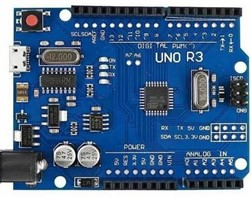
\includegraphics{Images/ArduinoUno.jpg}
    \caption{Board Arduino Uno R3}
    \label{fig:arduino}
\end{figure}
